\documentclass{article}

\usepackage[margin=1.0in]{geometry}
\usepackage{graphicx}
\usepackage{amsmath}
\usepackage{float}
\usepackage{enumitem}

\title{CSC 535 HW2}
\date{8/30/2018}
\author{Simon Swenson}

\begin{document}

\pagenumbering{gobble}
\maketitle
\pagenumbering{arabic}

\large Introduction

\small I completed all of the required homework problems. For some reason, 
fractions in tables are very small and slightly overlap other table elements. 
I think they are still readable, but I can provide the .tex source if you 
cannot read them.

\section{Q1}

\begin{tabular}{r | r r r r r r }
	  & 1 & 2 & 3 & 4 & 5 & 6 \\
	\hline
	1 & 2 & 3 & 4 & 5 & 6 & 7 \\
	2 & 3 & 4 & 5 & 6 & 7 & 8 \\
	3 & 4 & 5 & 6 & 7 & 8 & 9 \\
	4 & 5 & 6 & 7 & 8 & 9 & 10 \\
	5 & 6 & 7 & 8 & 9 & 10 & 11 \\
	6 & 7 & 8 & 9 & 10 & 11 & 12 \\
\end{tabular}

A clear pattern emerges along the diagonals.

\subsection{a}

Consider all outcomes where the sum is 6, that is, along the fifth diagonal of 
the chart above. There are five outcomes which sum to six, but only one of them 
is generated from a roll of two threes. Thus, $ P(A=3, B=3 | S=6) = 1/5 $.

\subsection{b}

There is only one cell in the chart where both $ A $ and $ B $ are three, and 
its sum is six. Thus: $ P(S=6 | A=3, B=3) = 1$.

\subsection{c}

Given a sum of six, there are no ways to get that from two ones, so 
$ P(A=1, B=1 | S=6) = 0 $.

\subsection{d}

There is only one cell where the sum is two, and it is certain that A is one, 
in that case. Thus, $ P(A=1 | S=2) = 1 $.

\subsection{e}

Given a sum of two, there are no ways to get that sum when A is three. Thus, 
$ P(A=3|S=2) = 0 $.

\subsection{f}

Given a sum of six, that is, five possibilities, there is only one way to get 
six when A is two, that is, when B is four. Thus, $ P(A=2|S=6) = 1/5 $.

\subsection{g}

In the whole chart, there is only one cell where the sum is 12, when both dice 
are six, so $ P(S=12) = 1/36 $.

\subsection{h}

A sum of six occurs five times in the chart, and the chart has 36 cells, so 
$ P(S=6) = 5/36 $.

\section{Q2}

\begin{tabular}{r r r | r }
	$a$ & $b$ & $c$ & $p(a, b, c) \times 1000 $\\
	\hline
	0 & 0 & 0 & 192 \\
	0 & 0 & 1 & 144 \\
	0 & 1 & 0 & 48 \\
	0 & 1 & 1 & 216 \\
	1 & 0 & 0 & 192 \\
	1 & 0 & 1 & 64 \\
	1 & 1 & 0 & 48 \\
	1 & 1 & 1 & 96 \\
\end{tabular}

Recall that marginalization over discrete values is: $ P(X) = \sum_Y P(X, Y) $. 
When we marginalize over c, we have the following table:

\begin{tabular}{r r | r }
	$a$ & $b$ & $p(a, b) \times 1000 $\\
	\hline
	0 & 0 & 336 \\
	0 & 1 & 264 \\
	1 & 0 & 256 \\
	1 & 1 & 144 \\
\end{tabular}

Also note the following probabilities:

\begin{align*}
    P(a = 0) \times 1000 &= 600 \\
    P(a = 1) \times 1000 &= 400 \\
    P(b = 0) \times 1000 &= 592 \\
    P(b = 1) \times 1000 &= 408 \\
\end{align*}

First, recall the definition for independence: $ P(A \cap B) = P(A) P(B) $.
Note that we only need one counter-example in $ A \times B $ to prove 
dependence. However, we prove that every scenario results in a contradiction:

\begin{align*}
    P(a = 0, b = 0) \times 1000 = 336 \ne 355.2 = 0.6 \times 0.592 \times 1000 &= P(a = 0) P(b = 0) \times 1000 \\
    P(a = 0, b = 1) \times 1000 = 264 \ne 244.8 = 0.6 \times 0.408 \times 1000 &= P(a = 0) P(b = 1) \times 1000 \\
    P(a = 1, b = 0) \times 1000 = 256 \ne 236.8 = 0.4 \times 0.592 \times 1000 &= P(a = 1) P(b = 0) \times 1000 \\
    P(a = 1, b = 1) \times 1000 = 144 \ne 163.2 = 0.4 \times 0.408 \times 1000 &= P(a = 1) P(b = 1) \times 1000 \\
\end{align*}

Now, let's condition the variables $ a, b $ on $ c $. Suppose $ c = 0 $. Then 
we have the following table (normalized):

\begin{tabular}{r r | c }
	$a$ & $b$ & $p(a, b | c = 0) $\\
	\hline
	0 & 0 & $ \frac{2}{5} $ \\
	0 & 1 & $ \frac{1}{10} $ \\
	1 & 0 & $ \frac{2}{5} $ \\
	1 & 1 & $ \frac{1}{10} $ \\
\end{tabular}

And corresponding probabilities:

\begin{align*}
    P(a = 0 | c = 0) &= \frac{1}{2} \\
    P(a = 1 | c = 0) &= \frac{1}{2} \\
    P(b = 0 | c = 0) &= \frac{4}{5} \\
    P(b = 1 | c = 0) &= \frac{1}{5} \\
\end{align*}

We can check that they are indeed conditionally independent:

\begin{align*}
    P(a = 0, b = 0 | c = 0) = \frac{2}{5} = \frac{1}{2} \times \frac{4}{5} &= P(a = 0 | c = 0) P(b = 0 | c = 0) \\
    P(a = 0, b = 1 | c = 0) = \frac{1}{10} = \frac{1}{2} \times \frac{1}{5} &= P(a = 0 | c = 0) P(b = 1 | c = 0) \\
    P(a = 1, b = 0 | c = 0) = \frac{2}{5} = \frac{1}{2} \times \frac{4}{5} &= P(a = 1 | c = 0) P(b = 0 | c = 0) \\
    P(a = 1, b = 1 | c = 0) = \frac{1}{10} = \frac{1}{2} \times \frac{1}{5} &= P(a = 1 | c = 0) P(b = 1 | c = 0) \\
\end{align*}

And a similar table supposing $ c = 1 $:

\begin{tabular}{r r | c }
	$ a $ & $ b $ & $ p(a, b | c = 1) $\\
	\hline
	0 & 0 & $ \frac{18}{65} $ \\
	0 & 1 & $ \frac{27}{65} $ \\
	1 & 0 & $ \frac{8}{65} $ \\
	1 & 1 & $ \frac{12}{65} $ \\
\end{tabular}

And corresponding probabilities:

\begin{align*}
    P(a = 0 | c = 1) &= \frac{9}{13} \\
    P(a = 1 | c = 1) &= \frac{4}{13} \\
    P(b = 0 | c = 1) &= \frac{2}{5} \\
    P(b = 1 | c = 1) &= \frac{3}{5} \\
\end{align*}

A similar check reveals that when conditioned on $ c = 1 $, $a, b$ 
are independent.

\begin{align*}
    P(a = 0, b = 0 | c = 1) = \frac{18}{65} = \frac{9}{13} \times \frac{2}{5} &= P(a = 0 | c = 1) P(b = 0 | c = 1) \\
    P(a = 0, b = 1 | c = 1) = \frac{27}{65} = \frac{9}{13} \times \frac{3}{5} &= P(a = 0 | c = 1) P(b = 1 | c = 1) \\
    P(a = 1, b = 0 | c = 1) = \frac{8}{65} = \frac{4}{13} \times \frac{2}{5} &= P(a = 1 | c = 1) P(b = 0 | c = 1) \\
    P(a = 1, b = 1 | c = 1) = \frac{12}{65} = \frac{4}{13} \times \frac{3}{5} &= P(a = 1 | c = 1) P(b = 1 | c = 1) \\
\end{align*}

\section{Q3}

\subsection{a}

~\\
~\\
~\\
~\\
~\\
~\\
~\\
~\\
~\\
~\\

\begin{figure}[!ht]
	\centering
	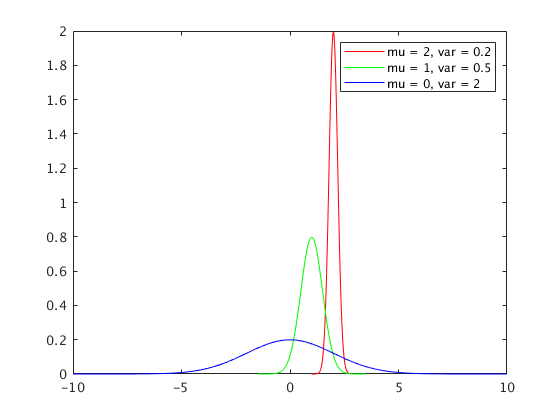
\includegraphics[width=100mm]{three-gaussians.png}
	\caption{Q3.a: Three Gaussian density functions with different means and standard 
deviations. The means define the centers of the humps. In addition, since these 
are probability density functions, the area under each one is one. A 
consequence of this is that when the standard deviation is smaller, the top of 
the curve gets higher. In other words, the narrower the hump of the curve is, 
the taller it must go to maintain an integral of one.}
\end{figure}

\subsection{b}

\begin{figure}[!ht]
	\centering
	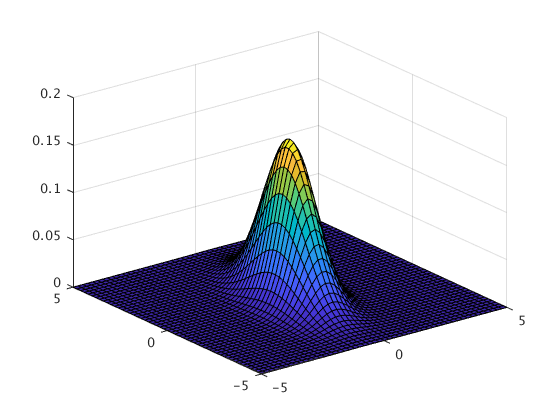
\includegraphics[width=100mm]{3d-gaussian.png}
	\caption{Q3.b: A 3D Gaussian distribution with a mean of [0, 0] and a covariance 
matrix of [0.5 0.3; 0.3 2.0]. Notice how the values in the covariance matrix 
affect the graph. In particular, the value at the bottom left of the covariance 
matrix is much higher than the other values. This affects the graph in the y 
direction, causing it to be much more gradual than the graph in the x 
direction. You can almost think of the diagonals of the covariance 
matrix as the variance in that graph's unit vector (x, y, etc.) 
direction. However, when multiple features (axes) are taken together, they can 
vary with each other, as well, hence we have a matrix instead of a vector.}
\end{figure}

\section{Q4}

Recall that, to find $ p(x) $ from a distribution $ p(x, y) $, we must 
marginalize y by the following: $ p(x) = \int_{-\infty}^{\infty} p(x, y) dy $. 
We can estimate such an integral by computing rectangular prisms for step 
values x and y (numerical integration). The expression is the following: 
$ sum(Z, 1) * s * s $, where Sum calculates the sum of each column (along 
the first axis), and s is the step size.

\begin{figure}[!ht]
	\centering
	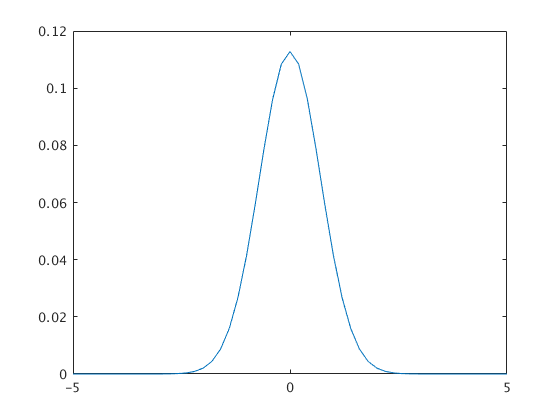
\includegraphics[width=100mm]{marginalized-gaussian.png}
	\caption{Q4: The estimation of $ p(x) $ by marginalizing $ y $. The graph 
appears to be another Gaussian distribution. This is not unexpected, but it is 
good to see that Gaussian distributions are well-behaved in this way.}
\end{figure}

~\\
~\\
~\\
~\\
~\\
~\\
~\\
~\\
~\\
~\\
~\\
~\\
~\\
~\\
~\\
~\\
~\\
~\\

\section{Q5}

We can use a similar technique as above. However, instead of summing the 
columns to marginalize over y, we pick a column where $ x = 0.5 $ (our prior), 
then norm that column.

\begin{figure}[!ht]
	\centering
	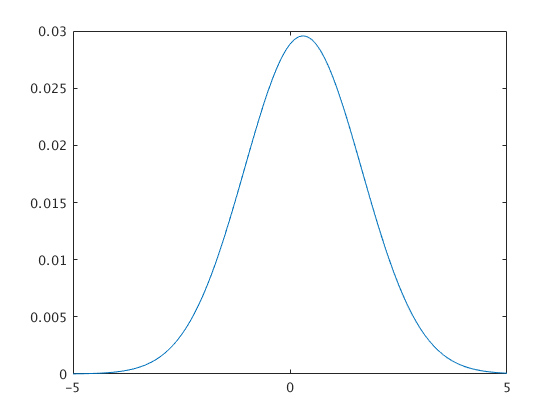
\includegraphics[width=100mm]{conditioned-gaussian.png}
	\caption{Q5: The estimation of $ p(y | x = 0.5) $. Given the output matrix 
of $ Z $ used to graph Q3.b, we can simply grab the column where $ x = 0.5 $ to 
become the new output values of our conditioned function. However, to ensure 
p sums to one, we must norm those values. Similar to Q4, the output is another 
Gaussian distribution. Thus, we see that both marginalization and conditioning 
a multivariate Gaussian distribution leads to another Gaussian distribtution.}
\end{figure}

\section{Q6}

\subsection{a}

\begin{enumerate}[label=\Alph*]
    \item $P(X|Y,Z)=P(X|Z) or P(Y,Z)=0$
    \item $P(Y|X,Z)=P(Y|Z) or P(X,Z)=0$
    \item $P(X,Y|Z)=P(X|Z)P(Y|Z)$
\end{enumerate}

\subsubsection{Proving B from A}

In layman's terms we would like to prove that, given $X$ is 
independent of $Y$, conditioned on $Z$, $Y$ is also independent of $X$, 
conditioned on $Z$. That is, conditional independence is \textit{symmetric}. 
This is intuitively obvious, but a proof is appreciated.
\begin{itemize}
    \item Let $X, Y, Z$ be sets of events.
    \item Suppose $P(X | Y, Z) = P(X | Z)$ or $P(Y, Z) = 0$, that is, $X$ is 
independent of $Y$, conditioned on $Z$.
    \item Ignore the case where $P(Y, Z) = 0$ to simplify the proof.
    \item Then $P(X | Y, Z) = P(X | Z)$
    \item $\Rightarrow \frac{P(X)P(Y,Z|X)}{P(Y,Z)} = \frac{P(X)P(Z|X)}{P(Z)}$ by Bayes's 
Rule.
    \item $\Rightarrow \frac{P(X)P(Z|X)P(Y|X,Z)}{P(Z)P(Y|Z)} = \frac{P(X)P(Z|X)}{P(Z)}$ by the chain rule.
    \item $\Rightarrow \frac{P(Y|X,Z)}{P(Y|Z)} = 1$ by algebra.
    \item $\Rightarrow P(Y|X,Z) = P(Y|Z)$ by algebra. QED.
\end{itemize}

\subsubsection{Proving C from A}

\begin{itemize}
    \item Suppose $P(X|Y,Z) = P(X|Z)$.
    \item $\Rightarrow \frac{P(X)P(Y,Z|X)}{P(Y,Z)} = P(X|Z)$ by Bayes's Rule.
    \item $\Rightarrow \frac{P(X)P(Y,Z|X)}{P(Z)P(Y|Z)} = P(X|Z)$ by the chain rule.
    \item $\Rightarrow \frac{P(X)P(Y,Z|X)}{P(Z)} = P(X|Z)P(Y|Z)$ by algebra.
    \item $\Rightarrow \frac{P(X)P(Y|X)P(Z|X,Y)}{P(Z)} = P(X|Z)P(Y|Z)$ by the chain rule.
    \item $\Rightarrow \frac{P(X,Y)P(Z|X,Y)}{P(Z)} = P(X|Z)P(Y|Z)$ by the inverse chain rule.
    \item $\Rightarrow P(X,Y|Z) = P(X|Z)P(Y|Z)$ by Bayes's Rule. QED.
\end{itemize}

\subsubsection{Proving A from C}

Unless I'm missing something catastrophic, here, this will just be the reverse 
of proving C from A, since all operations used have inverses. 
Consider the following:

\begin{itemize}
    \item Given $P(X,Y|Z) = P(X|Z)P(Y|Z)$
    \item $\Rightarrow \frac{P(X,Y)P(Z|X,Y)}{P(Z)} = P(X|Z)P(Y|Z)$ by Bayes's Rule.
    \item $\Rightarrow \frac{P(X)P(Y|X)P(Z|X,Y)}{P(Z)} = P(X|Z)P(Y|Z)$ by the chain rule.
    \item $\Rightarrow \frac{P(X)P(Y,Z|X)}{P(Z)} = P(X|Z)P(Y|Z)$ by the inverse chain rule.
    \item $\Rightarrow \frac{P(X)P(Y,Z|X)}{P(Z)P(Y|Z)} = P(X|Z)$ by algebra.
    \item $\Rightarrow \frac{P(X)P(Y,Z|X)}{P(Y,Z)} = P(X|Z)$ by the inverse chain rule.
    \item $\Rightarrow P(X|Y,Z) = P(X|Z)$ by Bayes's Rule. QED.
\end{itemize}

\section{Q7}

In this situation, we essentially have four scenarios, which broadly correspond 
to true positive, false positive, true negative, and false negative. If the sun 
hasn't exploded, but the instrument lies and tells us that it has, we have a 
false positive. If the sun has exploded, but the instrument lies and tell us 
that it hasn't, we have a false negative. I will examine the dice roll as one 
event rather than two, with probability $\frac{1}{36}$ that the instrument 
lies. Our prior of the probability of the sun exploding can greatly influence 
whether we believe that the instrument is telling the truth or not. For 
example, if that situation isn't very likely, the instrument could lie and give 
us false positives more often than it gives true positives.

\subsection{a}

If there is a $\frac{1}{6}$ chance of the sun exploding, there is also a 
$\frac{5}{6}$ chance of the sun \textit{not} exploding. Thus, we have the 
following:

\begin{tabular}{c | c}
	Event & Probability\\
	\hline
	Sun Explodes & $\frac{1}{6}$ \\
	Sun Doesn't Explode & $\frac{5}{6}$ \\
\end{tabular}

We can also consider the other event, the dice throw, in isolation as well:

\begin{tabular}{c | c}
	Event & Probability\\
	\hline
	Double Sixes & $\frac{1}{36}$ \\
	Any Other Roll & $\frac{35}{36}$ \\
\end{tabular}

When we introduce the two events to each other, we can better-understand the 
probabilities with a 2x2 chart:

\begin{tabular}{c | c c}
	  & Double Sixes & Any Other Roll \\
	\hline
	Sun Explodes & $\frac{1}{6} \times \frac{1}{36} = \frac{1}{216} \approx 0.00463 $ & $\frac{1}{6} \times \frac{35}{36} = \frac{35}{216} \approx 0.16204 $ \\
	Sun Doesn't Explode & $\frac{5}{6} \times \frac{1}{36} = \frac{5}{216} \approx 0.02315 $ & $\frac{5}{6} \times \frac{35}{36} = \frac{175}{216} \approx 0.81019 $ \\
\end{tabular}

The odds are then the lower-left quadrant to the upper-right quadrant:

$$
5:35
$$

or

$$
1:7
$$

Note that we assume that \textit{the two events are independent}. Here, we see 
that the sun exploding is likely enough to make the probability of a true 
positive (sun explodes, any other roll) higher than a false positive (sun 
doesn't explode, double sixes). Don't take this bet!

\subsection{b}

$\frac{1}{36}$ chance of the sun exploding. (I hypothesize that it will be 
dead even.)

\begin{tabular}{c | c c}
	  & Double Sixes & Any Other Roll \\
	\hline
	Sun Explodes & $\frac{1}{36} \times \frac{1}{36} = \frac{1}{1296} \approx 0.00077 $ & $\frac{1}{36} \times \frac{35}{36} = \frac{35}{1296} \approx 0.02701 $ \\
	Sun Doesn't Explode & $\frac{35}{36} \times \frac{1}{36} = \frac{35}{1296} \approx 0.02701 $ & $\frac{35}{36} \times \frac{35}{36} = \frac{1225}{1296} \approx 0.94522 $ \\
\end{tabular}

The odds are then the lower-left quadrant to the upper-right quadrant:

$$
35:35
$$

or

$$
1:1
$$

Even odds, as expected. If you're the gambling type, you might take this bet.

\subsection{c}

$\frac{1}{1000}$ chance of the sun exploding. Since $\frac{1}{36}$ was the 
critical point, I expect the false positives to now outweigh the true positives.

\begin{tabular}{c | c c}
	  & Double Sixes & Any Other Roll \\
	\hline
	Sun Explodes & $\frac{1}{1000} \times \frac{1}{36} = \frac{1}{36000} \approx 0.00003 $ & $\frac{1}{1000} \times \frac{35}{36} = \frac{35}{36000} \approx 0.00097 $ \\
	Sun Doesn't Explode & $\frac{999}{1000} \times \frac{1}{36} = \frac{999}{36000} = 0.02775 $ & $\frac{999}{1000} \times \frac{35}{36} = \frac{777}{800} \approx 0.97125 $ \\
\end{tabular}

The odds are then the lower-left quadrant to the upper-right quadrant:

$$
999:35
$$

Now, the false positives are vastly outweighing the true positives. Take the 
bet!

\subsection{d}

$\frac{1}{1000000}$ chance of the sun exploding.

\begin{tabular}{c | c c}
	  & Double Sixes & Any Other Roll \\
	\hline
	Sun Explodes & $\frac{1}{1000000} \times \frac{1}{36} = \frac{1}{36000000} \approx 0.00000 $ & $\frac{1}{1000000} \times \frac{35}{36} = \frac{35}{36000000} \approx 0.00000 $ \\
	Sun Doesn't Explode & $\frac{999999}{1000000} \times \frac{1}{36} = \frac{999999}{36000000} \approx 0.02778 $ & $\frac{999999}{1000000} \times \frac{35}{36} = \frac{777777}{800000} \approx 0.97222 $ \\
\end{tabular}

The odds are then the lower-left quadrant to the upper-right quadrant:

$$
999999:35
$$

or

$$
142857:5
$$

Here, the probability of the sun exploding dominates the equation, and my five 
digit decimal approximations were rounded to 0 for the sun exploding. This 
isn't surprising, considering the magnitude of one million. We can see that the 
false positive rate is now much, much higher than the true positive rate.

\end{document}